\documentclass[parskip=half]{scrartcl}

\usepackage[utf8]{inputenc}
\usepackage[ngerman]{babel}
\usepackage{amsmath}
\usepackage{amsfonts}
\usepackage{amssymb}
\usepackage{color}
\usepackage{hyperref}
\usepackage{graphicx}
\usepackage{epstopdf}
\usepackage{listings}
\usepackage{fancyvrb}
\definecolor{lnkcol}{rgb}{0.0,0.0,0.6}
\hypersetup{
	pdfstartview=FitH,
	colorlinks=true,
	urlcolor=lnkcol,
	citecolor=lnkcol,
	linkcolor=lnkcol,
	filecolor=lnkcol
}

\title{PiratenID: Technische Dokumentation}
\author{Jan Schejbal}
\date{}

\bibliographystyle{unsrt}

\setcounter{secnumdepth}{2}

\begin{document}
\maketitle

\begin{abstract}Dieses Dokument beschreibt das PiratenID-System sowie das darin verwendete Protokoll.
Es ist relevant für Personen, die die PiratenID-Software nachvollziehen, analysieren oder modifizieren wollen,
für Entwickler, welche einen eigenen Client programmieren möchten, sowie für technisch Interessierte, welche einen Blick hinter die Kulissen werfen möchten.
Gewöhnliche Nutzer des ID-Systems benötigen dieses Dokument nicht und sollten stattdessen die Anleitung für Nutzer\footnote{TODO} lesen.
Entwickler von Webanwendungen, die das PiratenID-System mittels fertiger Libraries nutzen möchten, müssen dieses Dokument nicht lesen,
können dies aber tun, um einen Einblick in Sicherheitsmaßnahmen bei Webanwendungen und ein besseres Verständnis des Systems zu erhalten.
Für Entwickler von Webanwendungen existiert eine separate Anleitung\footnote{TODO}, die die wichtigsten Punkte zusammenfasst.
\end{abstract}

\newpage

\tableofcontents

\newpage

\section{Einführung}
Das PiratenID-System soll es Mitgliedern der Piratenpartei ermöglichen, ihren Mitgliedschaftsstatus gegenüber von Dritten betriebenen Webseiten nachzuweisen,
ohne dass Zugriff auf die Mitgliederdatenbank nötig ist und ohne mehr Daten als nötig offenlegen zu müssen.

An einem Authentifizierungsvorgang sind immer drei Parteien beteiligt: Der Nutzer bzw. sein Browser, der Server des ID-Systems und die Webanwendung,
beispielsweise ein von Dritten betriebenes Forum oder Umfragetool.
Um Verwirrung zu vermeiden, wird der Begriff "`Client"' hier nicht verwendet, da dieser sowohl den Browser als auch die Webanwendung (Client des ID-Systems) bezeichnen könnte.
Die Parteien werden im Folgenden als ID-System, Browser und Webanwendung bezeichnet.

\section{Protokoll}
Nach Analyse vorhandener Verfahren, unter anderem X.509-Clientzertifikate, OpenID, SAML, OAuth sowie Protokollen mit kryptographisch gesicherter Anonymität/Pseudonymität
wurde entschieden, ein eigenes Protokoll zu entwickeln.
Der Hauptgrund dafür war, dass OpenID und SAML äußerst komplex sind und diese Komplexität Sicherheitsrisiken birgt sowie die Anwendung erschwert.
OpenID erfordert beispielsweise die Nutzung einer komplexen Library, und in gängigen Libraries
\footnote{Beispiel: Die PHP-OpenID-Library von Janrain greift bei fehlendem curl auf fopen zurück, was SSL-Zertifikate nicht prüft}
und OpenID-Servern\footnote{von Janrain betriebener Service, clickjacking bei inaktivem Javascript} wurden Sicherheitslücken entdeckt.
Das Protokoll sollte daher möglichst einfach sein, um eine Implementierung in beliebigen Programmiersprachen sowie eine Analyse zu ermöglichen.
Zur Übersicht über die Überlegungen zu anderen Protokollen wird hier auf das englischsprachige Dokument
"`Building an authentication system under strict real-world constraints"'
\footnote{TODO LINK} von Jan Schejbal verwiesen.

Das Protokoll ist angelehnt an SAML.
ID-System und Webanwendung kommunizieren niemals direkt miteinander, sondern ausschließlich über den Browser mittels HTTPS-Requests.
\footnote{Dadurch wird das Problem von serverseitiger Software die unsichere HTTPS-Verbindungen aufbaut (siehe PHP) vermieden.}
Der Ablauf einer Authentifizierung wird in Abbildung \ref{fig:protokolldiagramm} gezeigt.

\begin{figure}[h]
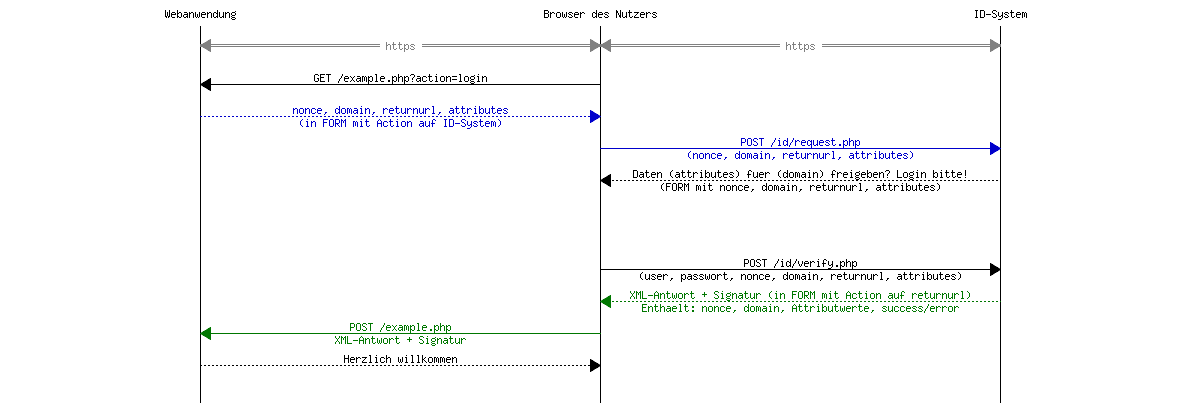
\includegraphics[trim=100px 0px 100px 0px, width=\textwidth]{protokolldiagramm.eps}
\caption{Ablauf einer Authentifizierung mit PiratenID}
\label{fig:protokolldiagramm}
\end{figure}

Wenn der Browser sich bei der Webanwendung einloggen möchte und die Loginseite aufruft, erhält er ein HTML-Form mit versteckten Formularfeldern.
In diesen sind enthalten:
\begin{itemize}
\item eine von der Webanwendung generierte Nonce (nicht vorhersagbare Zufallszahl zur Verhinderung von Replay-Attacken),
\item die Domain der Webanwendung,
\item die Return-URL (d.h. die Adresse an die das Ergebnis der Authentifizierungsanfrage gesendet wird)
\item die angefragten Attribute als mit Kommata getrennte Liste.
\end{itemize}

Die Nonce besteht aus 20-256 Zeichen, zulässige Zeichen sind Kleinbuchstaben, Großbuchstaben, Zahlen sowie \verb@ ! . : ; | / + _ -@.
Sie muss von der Webanwendung an die Sitzung des Nutzers gebunden gespeichert und beim Erhalt der Antwort geprüft werden.
Sie ist wie eine Session-ID dritten gegenüber geheim und nicht vorhersagbar zu halten.

Die Domain wird bei der Authentifizierung angezeigt und muss exakt zur Domain in der Return-URL passen.
Pseudonyme werden abhängig von der Domain berechnet.
Die Domain wird separat abgefragt, um ggf. später Ausnahmen zulassen zu können
(z. B. wenn eine Webanwendung umzieht, könnte eine Ausnahme eingerichtet werden um trotz neuer Domain in der Return-URL die alte Domain zu akzeptieren,
um die Pseudonyme migrieren zu können) oder die Prüfung aufzuweichen (z. B. Subdomains in der Return-URL zulassen).

Die Attribute werden im Abschnitt \ref{attribute} erläutert.

Nachdem der Browser das Formular mit diesen Werten erhalten hat, sendet er es (entweder automatisch per JavaScript oder manuell) per HTTPS-POST an das ID-System.
Dadurch wird der Nutzer auf die Seite des ID-Systems geleitet.
Die Seite zeigt, welche Daten an welche Domain übermittelt werden sollen, und enthält die Formularfelder erneut als verstecktes Formular.
Stimmt der Nutzer der Übertragung zu, bestätigt er dies mit seinem Benutzernamen und Kennwort und sendet das Formular per HTTPS-POST an das ID-System.

Das ID-System prüft die Zugangsdaten und erstellt eine XML-Antwort (Beispiel siehe Abbildung \ref{fig:xmlantwort}, das Format der Werte kann vom Live-System abweichen!).
Diese enthält die Nonce, die Domain, den Typ der Antwort (Erfolg/Fehler) sowie im Erfolgsfall die Attributwerte und im Fehlerfall eine Fehlerbeschreibung.
(Nur bei bestimmten Fehlern, z. B. Benutzerabbruch, wird eine Antwort gesendet.)
Die XML-Antwort wird daraufhin mit dem privaten Schlüssel des Servers signiert.
Die Antwort und Signatur werden (jeweils base64-encoded, um eine Beschädigung beim Transport zu vermeiden) in einem HTML-Form an den Browser zurückgeschickt.
Der Browser sendet dieses (entweder automatisch per JavaScript oder manuell) per HTTPS-POST an die Return-URL.


\newcommand\xmltag[1]{\textcolor[rgb]{0.00,0.00,0.70}{\textbf{#1}}}
\begin{figure}[h]
\small\begin{Verbatim}[commandchars=\\\{\}, ]
\xmltag{<?xml version="1.0"?>}
\xmltag{<PiratenIDResponse>}
    \xmltag{<nonce>}4e65731e9a097033c7e87d86b7d278c6acaf401e044c10907e93c17bf50cd631\xmltag{</nonce>}
    \xmltag{<domain>}localhost.janschejbal.de\xmltag{</domain>}
    \xmltag{<type>}success\xmltag{</type>}
    \xmltag{<attribute>}
        \xmltag{<name>}pseudonym\xmltag{</name>}
        \xmltag{<value>}d36a5e0e747a20ed5c2d42dd44666bb90ab6a7ca082f3598a1f548d6215fe673\xmltag{</value>}
    \xmltag{</attribute>}
    \xmltag{<attribute>}
        \xmltag{<name>}mitgliedschaft-bund\xmltag{</name>}
        \xmltag{<value>}Ja\xmltag{</value>}
    \xmltag{</attribute>}
    \xmltag{<attribute>}
        \xmltag{<name>}mitgliedschaft-land\xmltag{</name>}
        \xmltag{<value>}HE\xmltag{</value>}
    \xmltag{</attribute>}
\xmltag{</PiratenIDResponse>}
% \end{Verbatim}
\caption{Beispiel für eine XML-Antwort}
\label{fig:xmlantwort}
\end{figure}

Dort empfängt die Webanwendung die Daten und wertet sie aus. Zunächst wird die Gültigkeit der Signatur geprüft. Ist diese ungültig, werden die Daten verworfen.
Im Anschluss wird geprüft, ob die Nonce korrekt ist, d.h. einer von diesem Browser gestellten Authentifizierungsanfrage entspricht und noch nicht verwendet wurde,
sowie, ob die genannte Domain mit der eigenen Domain übereinstimmt. 
(Dies verhindert, dass ein Angreifer der eine andere Webanwendung betreibt, eine empfangene Antwort verwenden kann, um sich bei anderen Diensten als der Nutzer anzumelden.)
Die Nonce wird als verwendet markiert.

Danach wird geprüft, ob es sich um eine Erfolgsmeldung handelt.
Wenn ja, hat sich ein Nutzer erfolgreich eingeloggt - das heißt aber noch nicht, dass er ein Piratenmitglied ist, nur, dass er einen Account hat (den jeder haben kann)!
Um die Pirateneigenschaft zu prüfen, muss das Attribut "`mitgliedschaft-bund"' angefragt und verglichen werden. (Siehe Abschnitt \ref{attribute}).

\section{Attribute}\label{attribute}
Attribute sind Angaben über den eingeloggten Benutzer, die von der Webanwendung angefragt und mit Zustimmung des Nutzers vom ID-System mitgeteilt und bestätigt werden.
Die Attribute fallen in drei Kategorien, die im Folgenden erläutert werden.

\subsection{Pseudonym}
\label{sec:pseudo}
Das Pseudonym (Attributname \texttt{pseudonym}) ermöglicht es einer Webanwendung, einen Benutzer wiederzuerkennen.
Es handelt sich hierbei nicht um einen vom Nutzer gewählten Namen, sondern um einen berechneten Wert.

Zu jedem Benutzer wird in der Datenbank ein Zufallswert gespeichert, das sogenannte Usersecret. 
Das Pseudonym ist ein SHA256-Hash über eine systemweite geheime Konstante (das Pseudonym-Secret), das Usersecret sowie die anfragende Domain.
Ändert sich einer dieser Werte, ändert sich auch das Pseudonym.
Das Pseudonym ist somit für jede Kombination von Benutzer und Domain einmalig, d.h. ein Nutzer hat für jede Domain ein anderes Pseudonym.
Das konstante Pseudonym-Secret wäre hierbei eigentlich nicht nötig, erhöht aber die Sicherheit:
Wenn ein Angreifer Lesezugriff auf die Datenbank erhält, kann er ohne das (außerhalb der Datenbank) gespeicherte Pseudonym-Secret nichts mit den Usersecrets anfangen.
Versuche, die Hashes zu brechen und aus dem Pseudonym auf das Usersecret zu schließen sind bereits aufgrund der Entropie des Usersecrets aussichtslos.
Ohne Kenntnis von User- und Pseudonymsecret ist es nicht möglich festzustellen, ob zwei Pseudonyme dem gleichen Nutzer gehören.

Mit Zugriff auf die Secrets ist eine Zuordnung eines Pseudonyms zu einem Account möglich.
Bei einer Accountlöschung wird das Usersecret vernichtet, womit die Zuordnung nicht mehr möglich ist.

\subsection{Mitgliedschaften}
In den Attributen
\texttt{mitgliedschaft-bund}, \texttt{mitgliedschaft-land}, \texttt{mitgliedschaft-bezirk}, \texttt{mitgliedschaft-kreis} und \texttt{mitgliedschaft-ort}
wird festgehalten, in welchen Gliederungen eine Person Mitglied ist.

Diese Attribute sind nur ausgefüllt, wenn der Nutzer ein gültiges Token eingetragen hat.
Um zu prüfen, ob ein Nutzer Pirat ist oder nicht, muss das Attribut \texttt{mitgliedschaft-bund} abgefragt werden.
Nur wenn dort (TODO WERT) eingetragen ist, ist diese Person Mitglied.

Die übrigen Felder geben an, in welchen Untergliederungen der Nutzer Mitglied ist.
Für mögliche Werte sei auf die Liste der Untergliederungen\footnote{TODO} verwiesen.

Die Verknüpfung des Useraccounts mit den zugehörigen Daten findet über das Token statt.
Die Betreiber des ID-Servers können einen Account also nicht einer bestimmten Person zuordnen,
da die Zuordnung zwischen Token und Person nur über die Mitgliederverwaltung möglich ist.

\subsection{Personenbezogene Daten}
Auf Wunsch einiger Mitglieder wurde die Option vorgesehen, auch personenbezogene Daten über das ID-System bestätigen zu können.
Hierzu wurden die Attribute \texttt{realname} und \texttt{mitgliedsnummer} sowie entsprechende Datenbankfelder reserviert.

Über ein zweites Token ("`B-Teil"') könnten diese Werte nach einem noch festzulegenden Verfahren
nach ausdrücklicher und freiwilliger Zustimmung des Mitglieds aus der Mitgliederverwaltung nachgetragen werden.
Der Zugriff auf diese Attribute ist derzeit vollständig deaktiviert.
Nach der Aktivierung ist eine Whitelist vorgesehen, d.h. nur gesondert freigeschaltete Domains hätten die Möglichkeit, diese Daten anzufordern.
Diese Freischaltung würde nur für Webanwendungen erfolgen, die die Daten zwingend brauchen und strenge Datenschutzvorschriften einhalten.
Wie alle Attribute werden diese Informationen nur nach ausdrücklicher Zustimmung des Nutzers an einen Dienst herausgegeben.

Die Möglichkeit, diese Daten zu speichern, wird nicht aktiviert, bevor ein entsprechender Bedarf vorliegt, d.h. eine Anwendung existiert die diese Daten zwingend benötigt.
Für die meisten Webanwendungen sind diese Daten nicht erforderlich.

Der Großteil der IT möchte diese Daten \textbf{nicht} im System haben.


\section{Sicherheitseigenschaften}
In diesem Abschnitt werden Sicherheitseigenschaften des Systems aufgelistet, sowie die Maßnahmen genannt, die diese Eigenschaften sicherstellen.

\subsection{Nicht geplante Sicherheitseigenschaften}
Bevor auf die Sicherheitseigenschaften des Systems eingegangen wird, sollte erwähnt werden, welche möglichen Erwartungen an das System \textbf{nicht} erfüllt werden.
Die Liste kann logischerweise nie vollständig sein, sollte aber die wichtigsten Punkte umfassen.

\subsubsection{Ahsolute Sicherheit der Accounts}
Wie bei Onlinediensten üblich kann unter Angabe der E-Mail-Adresse eine Mail mit einem Kennwortrücksetzlink angefordert werden.
Ist ein Angreifer in der Lage, diese Mail mitzulesen, beispielsweise indem er den SMTP-Datenverkehr abhört oder Zugang zum E-Mail-Postfach des Nutzers hat,
kann er sich Zugang zum betroffenen Benutzerkonto verschaffen.

Dieses Risiko wird akzeptiert, da die Einschränkung der Nutzbarkeit ohne eine solche Funktion zu hoch wäre und es sich um ein allgemein übliches Verfahren handelt.
Angriffe, die auf dem Abhören der Mail bis zur Einlieferung ins Postfach des Empfängers beruhen, sind sehr selten.
Nutzer werden besonders darauf aufmerksam gemacht, dass sie den Zugang zu ihrem Postfach schützen müssen.

\subsubsection{Verwendete Mailadressen}
Da pro E-Mail-Adresse nur ein Benutzerkonto erstellt werden kann, kann beim Versuch einen Account anzulegen anhand der Fehlermeldung festgestellt werden,
ob mit der angegebenen Adresse bereits ein Benutzerkonto existiert.
Es wäre zwar möglich, dies zu verhindern, indem bei bereits verwendeter Adresse auch eine Erfolgsmeldung angezeigt wird und der Nutzer per Mail benachrichtigt wird.
Dies würde weiterhin erfordern, dass beim Zurücksetzen vergessener Kennwörter der Nutzer kein Feedback bekommt, wenn er eine falsche Adresse eingegben hat.
Eine solche Regelung wäre für den Nutzer verwirrend, und würde unter Umständen keine vollständige Sicherheit bieten (Seitenkanalangriffe).

Die Möglichkeit festzustellen, dass eine Adresse verwendet wird, wird daher akzeptiert,
was im Übrigen auch gängige Praxis
\footnote{getestet: wordpress.com (Passwortreset), drupal.org (Accounterstellung), phpbb.com (Accounterstellung im Supportforum, news.piratenpartei.de (Accounterstellung)}
ist.

\subsubsection{Schutz vor Betreiber}
Das System ist ein zentralisiertes Authentifizierungssystem.
Die Sicherheit beruht auf der Annahme, dass der Betreiber des Systems vertrauenswürdig ist.
Mit Zugriff auf den Signaturschlüssel können falsche XML-Antworten mit beliebigen Attributen erzeugt werden.
Der Betreiber hätte somit die Möglichkeit, sich mit fremden oder falschen Attributen bei Diensten zu identifizieren.
Der ID-Server sieht bei jedem Login-Vorgang, welcher Nutzer sich wann bei welchem Dienst angemeldet hat.
Mit den Daten des ID-Servers können mit realistischem Aufwand Pseudonyme zu Nutzern zugeordnet werden, solange das Usersecret nicht gelöscht wurde.

\subsubsection{Fehler beim Nutzer}
Das ID-System nutzt gewöhnliche Passwortauthentifizierung.
Wenn ein Nutzer ein unsicheres Passwort wählt oder es nicht geheim hält, kann jemand der dieses Passwort errät oder erlangt den Account missbrauchen.
Schadsoftware auf dem Rechner eines Nutzers kann das Kennwort ausspähen und den Account dieses Nutzers missbrauchen.
Das ID-System kann dem Nutzer die Pflicht nicht abnehmen, sich um seine Sicherheit zu kümmen. Hinweise auf Sicherheitsmaßnahmen werden jedoch gegeben.
Passwortrichtlinien (min. 8 Zeichen, min. 2 Arten von Zeichen) sind vorhanden.

Der Nutzer wird von fremden (d.h. potentiell bösartigen) Seiten auf die Seite des ID-Systems geleitet, wo er sich anmelden soll.
Der Nutzer muss selbst prüfen, dass er sich auf der richtigen Seite befindet.
Tut er dies nicht und gibt seine Nutzerdaten auf einer gefälschten Seite ein, können diese missbraucht werden.
Entsprechende Hinweise werden auf der Seite eingeblendet.
Die Verwendung von Spezialhardware (SecurID-Token, Smartcards) würde diese Probleme reduzieren, erscheint aber nicht angemessen.

\subsubsection{Sicherheitslücken in Webanwendungen}
Das ID-System schützt nicht vor Sicherheitslücken in den Webanwendungen.
Ist eine Webanwendung unsicher, kann sie die Daten ihrer Nutzer offenlegen oder Missbrauch der Anwendung zulassen.
Für die Entwickler von Webanwendungen steht ein Leitfaden zur Verfügung, der auch Sicherheitsthemen beinhaltet.
Die Entwickler sind für die Sicherheit der Anwendungen jedoch selbst verantwortlich.

\subsection{Vorgesehene Sicherheitseigenschaften}
\subsubsection{Sicherheit der Authentifizierung}
Bei korreter Anwendung des Protokolls soll sich die Webanwendung darauf verlassen können,
dass genau der Nutzer, zu dem die übermittelten Daten gehören, sich gegenüber dem ID-System eingeloggt hat,
sowie dass diese Daten korrekt sind.
Daraus folgt auch, dass es keinem Dritten möglich sein darf, sich mit einem fremden Pseudonym gegenüber einer Domain auszuweisen.

Die digitale Signatur über die Antwort stellt sicher, dass nur unverfälschte Antworten, die vom ID-System erstellt wurden, akzeptiert werden.
Die Nonce verhindert Replay-Attacken (eine Antwort auf eine andere Anfrage wird nicht akzeptiert, weil sie eine andere Nonce enthält).
Die verschlüsselte Übertragung der Daten stellt sicher, dass die signierte Antwort nicht von Unbefugten missbraucht werden kann.

Man-in-the-Middle-Attacken, bei denen eine Webanwendung die signierte XML-Antwort eines Nutzers missbraucht,
um sich als dieser Nutzer an einer anderen Domain anzumelden, werden ebenfalls verhindert:
Die Antwort enthält die Domain, für die sie gültig ist - weicht diese ab, wird die Antwort nicht akzeptiert.
(Ohne diese Prüfung könnte ein Angreifer der Zielanwendung gegenüber als Client auftreten, die Nonce dann dem Nutzer, der sich bei ihm anmeldet, weiterreichen,
und dann die ID-System-Antwort des Nutzers an die Zielanwendung schicken.)


\subsubsection{Vertraulichkeit der Daten}
Die freigegebenen Daten werden nur an den angegebenen Dienst herausgegeben.
Dies wird sichergestellt, indem die Domain, an die die Daten weitergegeben werden sollen, angezeigt wird,
und die Return-URL (an die die Daten gesendet werden) zu dieser Domain gehören muss.
Die Übertragung der Daten findet SSL-gesichert statt, sodass Dritte nicht mitlesen können.

Der Dienst, der die Daten erhält, kann technisch nicht daran gehindert werden, diese Daten zu missbrauchen oder weiterzugeben.
Der Nutzer muss selbst entscheiden, ob er einem Dienst seine Daten anvertrauen möchte.

\subsubsection{Datenweitergabe nur mit Einverständnis}
Im ID-System gespeicherte Daten werden nur mit Einverständnis des Nutzers, bestätigt durch die Eingabe des Kennworts, weitergegeben.

\subsubsection{Ein Pirat - ein Pseudonym (pro Domain)}
Jeder Nutzer hat nur ein Pseudonym pro Domain.
Eine Webanwendung, die Umfragen oder Abstimmungen anbietet, kann sich daher in der Regel darauf verlassen, dass jedes Mitglied nur einmal teilnehmen kann,
wenn pro Pseudonym nur eine Teilnahme ermöglicht wird und die Mitgliedseigenschaft geprüft wird.

Aus diesem Grund ist es einem Teilnehmer auch nicht möglich, sein Pseudonym zu ändern, allerdings kann jeder mehrere Benutzerkonten haben.
Die Bindung eines Kontos an eine Person geschieht erst durch die Eingabe eines Tokens - ohne Token ist das Konto nicht als das Konto eines Mitglieds bestätigt.
Um sicherzustellen, dass ein Mitglied (in seiner Eigenschaft als Mitglied) nicht mehrere Konten (und somit mehrere Pseudonyme nutzt),
wird bei der Eingabe eines Tokens dieses an das entsprechende Konto gebunden.

Ein einmal eingegebenes Token kann nicht mehr entfernt oder geändert werden, und es ist nicht möglich, das gleiche Token für ein anderes Konto zu verwenden.
Wird ein Benutzerkonto gelöscht, bleibt das Token (bzw. ein Hash davon) gespeichert, um sicherzustellen, dass es nicht wiederverwendet werden kann
(ein neues Konto hätte ein anderes Usersecret und somit andere Pseudonyme).

Da mit der Löschung eines Kontos bis auf das Token alle Daten (inkl. Usersecret) gelöscht werden, und ein Token nicht wiederverwendet werden kann,
bedeutet dies, dass ein Mitglied, welches sein Konto mit eingetragenem Token löscht, das ID-System nicht mehr benutzen kann.
Die Mitgliederverwaltung darf in diesem Fall \textbf{kein} neues Token ausstellen, da das Prinzip "`Ein Pirat - ein Pseudonym"' damit verletzt würde!

Nicht verwendete Token können beliebig ausgetauscht werden. Vor der Neuausstellung eines Tokens sollte die Mitgliederverwaltung bestätigen lassen,
dass das alte Token nicht verwendet wurde.
Sollte ein Austausch verwendeter Token gewünscht sein, muss entweder die Verletzung dieses Prinzips im Einzelfall in Kauf genommen werden,
oder es muss ein weiteres Attribut "`token-index"' eingeführt werden, durch welches Webanwendungen gegenüber angezeigt wird, ob ein Token neu ausgestellt wurde.
Webanwendungen könnten somit selbst entscheiden, ob bzw. bis zu wie viele Neuausstellungen (d.h. Pseudonymänderungen) sie pro Mitglied zulassen.


\subsubsection{Nichtverknüpfbarkeit der Pseudonyme}
Es soll Dritten nicht möglich sein, Pseudonyme mit dem Benutzerkonto oder mit anderen Pseudonymen zu verknüpfen,
d.h. es soll auch zusammenarbeitenden Diensteanbietern (mit verschiedenen Domains) nicht möglich sein festzustellen, 
dass ein Pseudonym zu einem bestimmten Benutzerkonto gehört oder dass
Pseudonym 1 in der ersten Webanwendung und Pseudonym 2 in der zweiten Webanwendung dem gleichen Nutzer gehören.
Dies wird durch das Berechnungsverfahren für Pseudonyme (siehe entsprechender Abschnitt) sichergestellt.


\subsection{Vermutete Sicherheitseigenschaften}
Die im folgenden benannten Eigenschaften sind während der Entwicklung "`nebenbei"' entstanden und wurden nicht vollständig überprüft.
Es handelt sich um zusätzliche Eigenschaften die keineswegs für einen sicheren Betrieb nötig sind, jedoch die Sicherheit erhöhen können
(Defence in depth) oder technisch interessant sind.

\subsubsection{Stärke gegen Angreifer mit Datenbankzugriff}
Ein Angreifer, der Lesezugriff auf die (gegen solchen Zugriff selbstverständlich geschützte) Datenbank erlangt,
kann zwar die Nutzerdatenbank auslesen, aber nicht am System missbrauchen.
Insbesondere sollte es nicht möglich sein, ein benutzbares Token zu erhalten (da die Token gehasht gespeichert werden, aber im Klartext eingegeben werden müssen),
ein Benutzerkonto zu nutzen/übernehmen (da die Passwörter gehasht gespeichert werden),
ein Kennwort zurückzusetzen (Reset-Keys werden gehasht gespeichert) oder
eine falsche E-Mail-Adresse zu bestätigen (Bestätigungskeys werden gehasht gespeichert).
Auch bei einem unsicheren Kennwort sollte der Angreifer keine Möglichkeit haben, den Passworthash zu Bruteforcen,
da ein zusätzliches, in den Systemkonstanten gespeichertes geheimes Salt verwendet wird.
(Die Möglichkeit einer langsamen und somit nur gegen sehr schwache Kennwörter möglichen Online-Bruteforce-Attacke bleibt unverändert.)

Auch das Zuordnen von Pseudonymen sollte unmöglich sein, da das zusätzlich verwendete Pseudonym-Secret unbekannt ist.

\subsubsection{Stärke gegen Angreifer mit Dateisystemzugriff}
Ein Angreifer, der Lesezugriff auf das Dateisystem erlangt, ist in der Lage, den Signaturkey auszulesen und somit falsche XML-Antworten zu erzeugen.
Ohne vorherige Kenntnis des Pseudonyms kann er dieses nur berechnen (und darüber Pseudonyme zuordnen),
wenn er auch Zugriff auf die Datenbank (oder die Dateien in der die Datenbanktabellen liegen) hat.
Ohne Kenntnis des Pseudonyms kann er gegenüber Webanwendungen nicht vortäuschen, ein bestimmter anderer Nutzer zu sein.
Benutzerkonten mit sicheren Kennwörtern sollten weiterhin wie beim Angreifer mit Datenbankzugriff geschützt sein.


\section{Schutzmaßnahmen gegen Angriffe}
\subsection{Server}
\subsubsection{Schwachstelle Mensch}
Um Angriffe, die Fehler des Nutzers ausnutzen, zu erschweren, werden die Nutzer durch gut sichtbare Werbebanner auf wichtige Sicherheitsmaßnahmen hingewiesen.
Dazu zählt die sichere Verwendung von HTTPS, Sicherheit des verwendeten Computers, Passwortsicherheit, sowie die Absicherung des E-Mail-Accounts.

\subsubsection{Cross-site request forgery, Session-basierte Angriffe}
Der Server des ID-Systems arbeitet vollständig ohne Sessions. CSRF sowie andere Session-basierte Angriffe sind somit nicht möglich.
Der Nutzer muss zur Bestätigung von Transaktionen jedes mal seine Logindaten eingeben.
Der Zugriff auf Nutzerdaten wird wo möglich über einer Funktion gekapselt, die die Logindaten prüft, um Programmierfehler auszuschließen.

\subsubsection{SQL-Injection/Truncation}
Zum Schutz vor SQL-Injection werden Prepared Statements benutzt.
Um Truncation-Angriffe zu verhindern, wird an mehreren Stellen die Länge von Parametern geprüft
und die Datenbankverbindung so konfiguriert (SQL mode), dass auch leichte Fehler (z. B. überlange Felder) als Fehler behandelt werden.

\subsubsection{Passwort-Hashverfahren}
\label{sec:pwhash}
Kennwörter werden nicht im Klartext, sondern mit SHA256 gehasht gespeichert.
Dabei werden der Benutzername als Salt, ein zusätzliches systemspezifisches Salt und strengthening als zusätzlicher Schutz eingesetzt.

Das bedeutet, dass ein Angreifer, der die Datenbank erlangt, zwar prüfen kann, ob ein Benutzer ein bestimmtes Kennwort hat,
die Kennwörter aber nicht entschlüsseln kann.
Der gängige Angriff gegen derart gesicherte Passwörter ist es, jedes Wort aus einer Liste (Wörterbuch, alle Buchstabenkombinationen, ...)
gegen die Liste zu prüfen, um so Treffer zu finden und Kennwörter aufzudecken (Brute-Force/Dictionary attack).

Um solche Angriffe zu erschweren, werden die Hashes folgendermaßen gebildet:
\begin{enumerate}
	\item Das Kennwort wird mit dem Benutzernamen (benutzerspezifisches Salt) und einer geheimen Systemkonstante (Systemsalt) verkettet und gehasht
	\item Der aktuelle Hash wird verkettet mit einem Zähler und dem ersten Hash, und erneut gehasht (das Ergebnis wird der neue aktuelle Hash).
	\item Dieser Schritt wird für viele Iterationen wiederholt (der Zähler wird jeweils hochgezählt)
\end{enumerate}

Die Salts sorgen dafür, dass das gleiche Kennwort bei zwei unterschiedlichen Nutzern oder auf zwei verschiedenen Systemen unterschiedliche Hashes ergibt.
Das geheime Systemsalt macht Angriffe gegen die Hashes völlig unmöglich, solange der Angreifer es nicht erlangt.
Die Verkettung und Verwendung des Zählers stellt sicher, dass jede Iteration anders ist und verhindert so, dass das Verfahren in einen Zyklus gerät.

Durch die Verwendung der Salts wird die Verwendung vorausberechneter Rainbow Tables zur Beschleunigung von Angriffen unmöglich.
Um ein Kennwort auf Gültigkeit zu testen, müssen zahlreiche Hashes (Iterationen) berechnet werden, was einige Millisekunden dauert.
Dadurch werden Brute-Force-Versuche so stark ausgebremst, dass sie unpraktisch werden.

Anzumerken ist, dass diese Schutzmaßnahmen nur für den unwahrscheinlichen Fall benötigt werden, dass es einem Angreifer gelingt, die Benutzerdatenbank zu kopieren.
Da die Verlangsamung durch das strengthening auch auf den Server selbst zutrifft,
wird auch bei Online-Brute-Force-Versuchen die Geschwindigkeit durch die CPU-Leistung des Servers wirksam begrenzt.

\subsubsection{Hashing}
Auch andere Informationen werden wo möglich nur gehasht gespeichert,
beispielsweise die Token und die zum Zurücksetzen von Passwörtern und Bestätigen von Mailadressen nötigen Keys.

\subsubsection{Clickjacking-Schutzmaßnahmen}
Bei webbasierten Diensten besteht die Gefahr des sogenannten Clickjackings.
Hierbei wird die angegriffene Website (hier: das ID-System) unsichtbar eingebunden, und der Nutzer dazu gebracht, eine (sichtbare) Schaltfläche zu drücken.
Der Klick auf die Schaltfläche trifft jedoch durch geschickte Anordnung der Elemente die angegriffene Webseite und löst dort eine Aktion aus.
Im Fall des ID-Systems könnte dies z. B. die Bestätigung der Datenfreigabe sein.

Auch der Zwang, zu jeder Aktion das Kennwort eingeben zu müssen, schützt nicht vor diesem Angriff, da viele Browser Kennwörter speichern und automatisch ausfüllen.
Um diesen Angriff zu verhindern, werden drei Schutzmaßnahmen getroffen:

Ein entsprechender HTTP-Header (\texttt{X-Frame-Options: deny}) verhindert in modernen Browsern die Einbettung.
Dies ist insbesondere deswegen wichtig, in modernen Browsern IFRAME-Attribute (z. B. \texttt{sandbox}) den Javascript-basierten Schutz aushebeln.

Nutzer ohne JavaScript müssen beim Login zufällige Ziffern abtippen, welche als ausformulierte Wörter mit zufälliger Position auf der Seite stehen.
Da bei Clickjacking die einbettende Seite nicht auf den Inhalt der eingebetteten Seite zugreifen kann, verhindert dies den Angriff weitgehend.
Die zufällige Positionierung verhindert, dass dieser Teil der Website sichtbar belassen und nur der Rest überdeckt wird.
Das Ausschreiben als Wort verhindert, dass der Nutzer dazu gebracht wird, die Ziffern zu markieren und ins Zielfeld zu ziehen.
Da sowohl vor als auch nach den Ziffern ein zufälliger Abstand eingefügt wird, kann ein Angriff auch aus der Länge der Webseite nicht die korrekte Position errechnen.

Bei aktivem JavaScript wird eine Einbettung erkannt und in einem solchen Fall eine Warnung angezeigt sowie die Seite des ID-Systems verborgen.

\subsubsection{Sichere Zufallszahlen}
Zufallszahlen, bei denen ein hohes Sicherheitsniveau erforderlich ist, werden über OpenSSL generiert, statt sich auf unsichere PHP-Methoden zu verlassen.
Dadurch ist die hohe Qualität und Nichtvorhersagbarkeit der Zufallszahlen sichergestellt.

\subsubsection{HTTPS}
Sämtliche Kommunikation mit dem ID-System erfolgt über HTTPS.
Um Nutzer, die versuchen, die Adresse mit "`http"' statt "`https"' einzugeben, zu schützen, wird der \texttt{Strict-Transport-Security}-Header genutzt.
Dieser weist moderne Browser an, die Seite ausschließlich über HTTPS abzurufen und verhindert so,
dass Nutzer es über HTTP versuchen und sich so der Gefahr von MitM-Attacken aussetzen.

\subsubsection{Internet Explorer 6}
Nutzer des Internet Explorer 6 und früher werden von der Nutzung des ID-Systems ausgeschlossen und darauf hingewiesen, dass sie ihr System aktualisieren sollen.
Mit dem IE6 ist eine sichere Internetnutzung nicht möglich, zudem deutet sein Vorhandensein auch auf ein generell veraltetes (und somit unsicheres) System hin.



TODO (client)
- session fixation
- session-cookie sicherheit
- selbstschutz gegen falsche verwendung
- anleitung

\section{Datenbank}
TODO
- zwei tabellen
- erklärung import
- erklärung felder

\section{Dateien des Servers}

\subsection{Verzeichnis /includes/}
Dieses Verzeichnis enthält Dateien, die von den anderen Skripten eingebunden werden.

\subsubsection{/includes/header.inc.php}
Diese Datei enthält den Anfang jeder ausgegebenen HTML-Seite und nimmt auch einige Einstellungen vor.
\begin{itemize}
	\item Ein Error-Handler, der Fehler wie Warnungen zu fatalen Fehlern macht und wenig Informationen über den Fehler mitteilt, wird aktiviert
	\item Es wird sichergestellt, dass \texttt{register\_globals} deaktiviert ist.
	\item \texttt{siteconstants.inc.php} und \texttt{functions-global.inc.php} werden eingebunden
	\item Die HTTP-Header \texttt{X-Frame-Options} und \texttt{Strict-Transport-Security}
	\item Das HTML-Grundgerüst der Seite mit Sicherheitshinweisen, Menü und IE6-Blocker wird ausgeliefert. Das maincontent-DIV wird geöffnet
\end{itemize}

\subsubsection{/includes/footer.inc.php}
Diese Datei enthält das Ende jeder ausgegebenen HTML-Seite:
\begin{itemize}
	\item Der IE6-Blocker und das maincontent-DIV werden geschlossen
	\item Die Fußzeile wird ausgegeben
	\item Der JavaScript-basierte Clickjacking-Schutz wird ausgegeben
\end{itemize}

\subsubsection{/includes/siteconstants.inc.php}
Diese Datei enthält (z.T. geheime!) Konstanten, die bei der Installation des Servers gesetzt werden müssen:
\begin{itemize}
	\item \texttt{\$sitepath} - Die absolute Adresse des ID-Systems. Wird z. B. beim Versand von E-Mails verwendet.
	\item \texttt{\$extendedAttributeDomains} - Die Liste der Domains, die erweiterte Attribute (Realname, Mitgliedsnummer) anfragen können.
	\item \texttt{getDatabasePDO()} - Hier werden die Datenbank-Zugangsdaten eingetragen
	\item \texttt{\$pseudonymsecret} - Ein zusätzliches Salt zur Berechnung der Pseudonyme, siehe Abschnitt \ref{sec:pseudo} Pseudonyme.
	\item \texttt{\$passwordsaltsecret} - Ein zusätzliches Salt zur Berechnung der Passwort-Hashes, siehe Abschnitt \ref{sec:pwhash} Passwort-Hashverfahren.
	\item \texttt{\$signaturekey\_pem} - Der private RSA-Signaturschlüssel, mindestens 2048 Bit.
		Wird dieser Schlüssel kompromittiert, muss er sofort getauscht und der alte Schlüssel in den Webanwendungen deaktiviert werden!
\end{itemize}
Maßnahmen, die zu treffen sind, wenn eine der geheimen Konstanten kompromittiert wird, sind in der Datei selbst dokumentiert.


\subsubsection{/includes/functions-global.inc.php}
Diese Datei enthält die globalen Funktionen:
\begin{itemize}
	\item \texttt{safeout(\&\$text)} - Gibt eine Variable mit korrektem HTML-Escaping aus. Ist die Variable undefiniert, wird nichts ausgegeben, aber keine Warnung erzeugt
	\item \texttt{prefilter(...)} - Prüft einen Wert (z. B. GET/POST-Parameter) auf Existenz, Typ und Länge
	\item \texttt{generateNonce(\$entropy)} - Erzeugt die angegebene Anzahl sicherer Zufallsbytes (Hex-encoded)
	\item \texttt{hashPassword(\$username, \$pw)} - Berechnet den Passwort-Hash, siehe Abschnitt \ref{sec:pwhash} Passwort-Hashverfahren
	\item \texttt{class DB} - Die DB-Klasse kapselt Datenbankzugriffe über ein Singleton.
	\begin{itemize}
		\item Die Felder connection, statement und error sind zwecks leichtem Zugriff public.
		\item \texttt{query(...)} führt eine Datenbankabfrage (mit Längenprüfung der Parameter) durch. Die Felder statement und ggf. error werden gesetzt.
		\item \texttt{get()} liefert die Singleton-Instanz
		\item \texttt{cleanup()} löscht veraltete Daten und wird automatisch beim Erstellen einer neuen Instanz aufgerufen
	\end{itemize}
	\item \texttt{getUser(...)} - Wenn in den POST-Variablen ein gültiges Login (inkl. Clickjacking-Schutz) liegt, wird der dazugehörige User mit allen Daten zurückgegeben.
	                           Zugriffe auf Benutzerdaten erfolgen über den Rückgabewert dieser Funktion, um sicherzustellen, dass immer ein Login erforderlich ist.
	\item \texttt{printLoginFields()} - Gibt Felder für ein Loginformular inkl. Clickjacking-Schutz aus (die mit getUser() kompatibel sind)
	\item \texttt{checkPassword(...)} - Prüft, ob ein Passwort inkl. Wiederholung in Ordnung sind, d.h. das Passwort setzt werden kann.
										Prüft \textbf{nicht} ob ein Login gültig ist, dafür ist getUser da!
	\item \texttt{checkMail(...)} - Prüft, ob eine E-Mail-Adresse gültig und noch nicht verwendet (d.h. für das Anlegen eines Accounts zulässig) ist
\end{itemize}

\subsubsection{/includes/.htaccess}
Diese Datei verhindert direkten Zugriff auf die Include-Files.



\subsection{Verzeichnis /user/}
Dieses Verzeichnis enthält Seiten, die mit der Verwaltung der Benutzerkonten zusammenhängen.

\subsubsection{/user/create.php}
Diese Datei regelt die Erstellung von Benutzerkonten.
Sie zeigt das entsprechende Formular an, nimmt die Daten entgegen, prüft sie, trägt den Nutzer in der Datenbank ein und versendet die Aktivierungsmail.

\subsubsection{/user/confirm.php}
Diese Datei regelt die Bestätigung der Mailadresse/Aktivierung der Benutzerkonten.
Sie wird ausschließlich über einen Link aus der Aktivierungsmail aufgerufen und erhält den Aktivierungsschlüssel.
Daraufhin versucht sie die Datenbank entsprechend zu aktualisieren und teilt dem Nutzer das Ergebnis mit.
Im Erfolgsfall wird (mit einem Link auf entertoken.php) darauf hingewiesen, dass der Nutzer jetzt sein Token eintragen soll.

\subsubsection{/user/entertoken.php}
Diese Datei ermöglicht es dem Nutzer, seinem Account ein Token hinzuzufügen.
Sie zeigt das entsprechende Formular an, nimmt die Daten entgegen, prüft sie und trägt die Änderung in der Datenbank ein.

\subsubsection{/user/changepw.php}
Diese Datei ermöglicht es dem Nutzer, sein Kennwort zu ändern.
Sie zeigt das entsprechende Formular an, nimmt die Daten entgegen, prüft sie und trägt die Änderung in der Datenbank ein.

\subsubsection{/user/requestreset.php}
Diese Datei ermöglicht es dem Nutzer, eine Passwortreset-Mail anzufordern.
Sie zeigt das entsprechende Formular an, nimmt die Daten entgegen, prüft sie, erstellt ggf. ein Token und trägt es in die Datenbank ein und verschickt die Mail mit dem Link.

\subsubsection{/user/reset.php}
Diese Datei ermöglicht es dem Nutzer, sein Kennwort über einen via requestreset.php angeforderten Link zurückzusetzen.
TODO

\subsubsection{/user/delete.php}
Diese Datei ermöglicht es dem Nutzer, sein Benutzerkonto zu löschen.
Sie zeigt das entsprechende Formular an, nimmt die Daten entgegen, prüft sie, und löscht ggf. das Konto.
Der Nutzer muss die Löschung durch Eingabe des Wortes LOESCHEN bestätigen.
Um den Account zu löschen, werden bis auf Token(hash), E-Mail-Verifizierungsstatus und Erstellungsdatum alle Daten überschrieben.
Der Tokenhash bleibt gespeichert, damit das Token nicht wiederverwendet werden kann.
Der Benutzername wird durch einen zufällig generierten Benutzernamen ersetzt.

\subsection{Verzeichnis /id/}
Dieses Verzeichnis enthält die serverseitige Implementierung des PiratenID-Protokolls.

TODO Document, review



\subsection{Verzeichnis /static/}
Dieses Verzeichnis enthält statische Dateien wie Grafiken, Stylesheets, die Sicherheits-Hinweisbanner etc.


\section{Datenbank}
Ein SQL-Dump der Datenbankstruktur sollte dieser Dokumentation beiliegen.
Die Datenbank besteht aus zwei Tabellen:

TODO





\end{document}




